\documentclass[11pt,letterpaper]{article}

\usepackage{fancyhdr}
\usepackage[latin1]{inputenc}
\usepackage{amsmath}
\usepackage{amsfonts}
\usepackage{amssymb}
\usepackage{graphicx}
\usepackage[hmargin=2cm,vmargin=2.5cm]{geometry}
\usepackage[normalem]{ulem}
\usepackage{enumerate}
\usepackage{hyperref}
\usepackage{palatino}

\newcommand{\workingDate}{\textsc{14 November 2014}}
\newcommand{\courseName}{MTH 201}
\newcommand{\institution}{Grand Valley State University}

\pagestyle{fancy}
\setlength\parindent{0in}
\setlength\parskip{0.1in}
\setlength\headheight{15pt}

%%%%%%%%%%% HEADER / FOOTER %%%%%%%%%%%
\rhead{\workingDate}
\chead{\textsc{Lab 10}}
\lhead{\textsc{\courseName}}
\rfoot{\textsc{\thepage}}
\cfoot{\textit{Built: \today}}
\lfoot{\textsc{\institution}}

\begin{document}

\begin{flushright}
	\begin{Large}
		Lab 8: Applying Riemann sums to estimate total change
	\end{Large}
\end{flushright}

\subsection*{Introduction and instructions} 

In this lab, we'll put what we've learned about Riemann sums into practice to reconstruct the total amount of change in a quantity if all we are given is its rate of change. 

During this lab, you'll be using a Desmos page to automate your Riemann sum calculations. This page is found at: 
\begin{center}
    \url{https://www.desmos.com/calculator/tgyr42ezjq} 
\end{center}
This special Desmos construction visualizes Riemann sums and calculates them for you. When you open this page, you will see several items in the left sidebar area, some of which you need to manipulate and others you need to ignore. Here is a guide: 

\begin{itemize}
    \item The first box is where you enter a formula for your function. You will need to use $x$ as the input variable, not $t$ or any other letter. 
    \item The sliders for left endpoint and right endpoint control where the left and right edges of the area you are estimating are. You'll need to change these if the situation calls for it. 
    \item The ``number of intervals'' slider controls the number of intervals, or the number of rectangles being used. 
    \item The ``choice of method'' slider has three options: select $c=0$ for left sums, $c=0.5$ for midpoint sums, and $c = 1$ for right sums. 
    \item The box with a large $\Sigma$ and the word ``integral approximation'' above it shows the value of the Riemann sum in the smaller box ``$I = $''. 
    \item You can ignore everything else; in fact don't touch anything else! 
\end{itemize}
For example, here is a screenshot showing that the area between the graph of $y = \cos(\sin(x)) -x $, the $x$-axis, and the bounds $x=0$ and $x=2$ is approximately $-0.556202755481$, using a midpoint Riemann sum with 8 rectangles:  
\begin{center}
    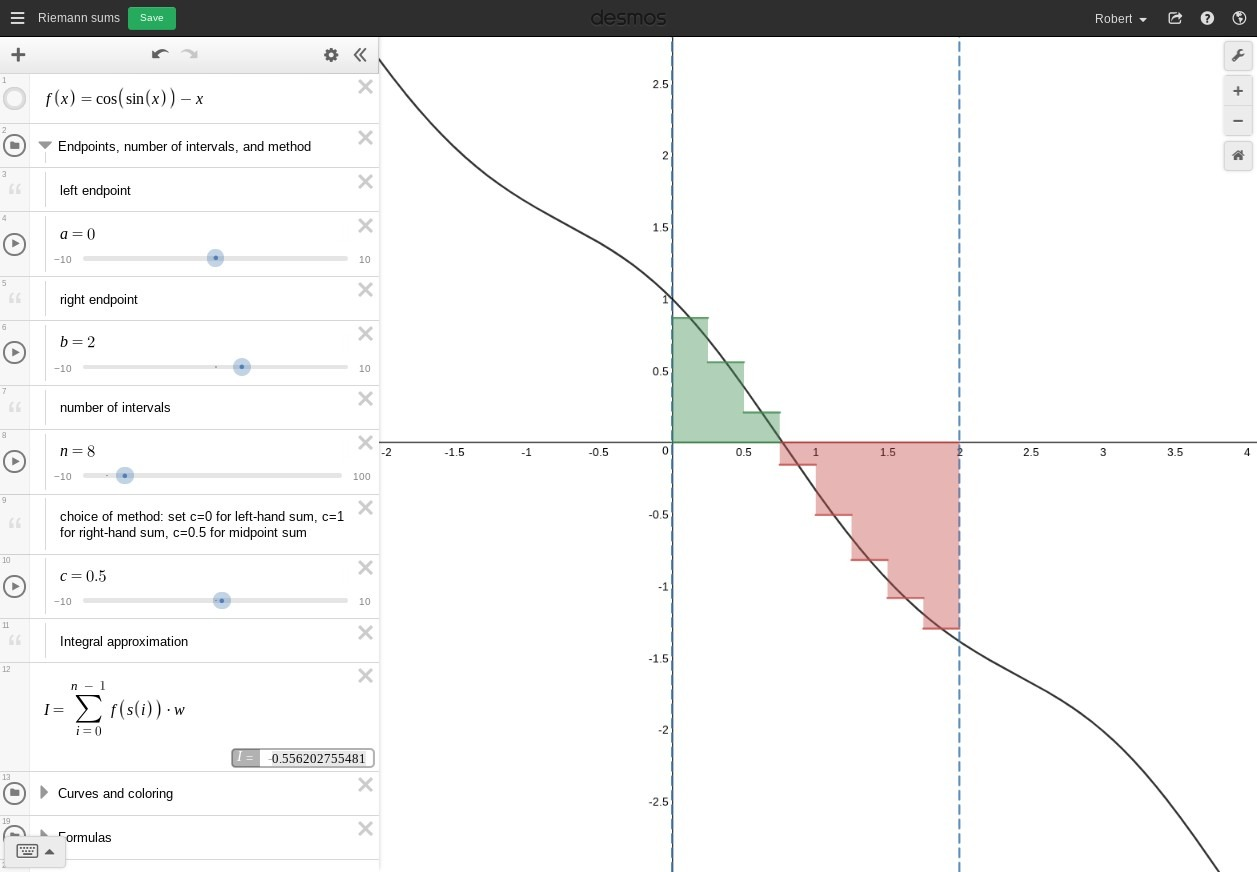
\includegraphics[width=5in]{riemann-example.jpeg}}
\end{center}
Note that positive area is shaded green and negative area is shaded red. 

% subsection overview (end)

\subsection*{Main Activity}

The rate at which pollution escapes a scrubbing process at a manufacturing plant increases over time as filters and other technologies become less effective. For this particular example, assume that the rate of pollution (in tons per week) is given by the function $r$ whose graph is given below: 

\begin{center}
	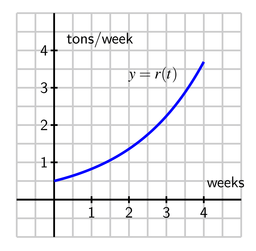
\includegraphics[width=0.25\textwidth]{lab10-plot_preview.png}
\end{center}

\begin{enumerate}
	\item Use the graph to estimate the value of $M_4$ on the interval $[0,4]$. Show all work and put correct units of measurement on your answer. 

	\item What does your answer from part (a) mean, in terms of the pollution discharged from the plant? Give your answer in one clear and correct sentence. 

	\item Now suppose that $r$ is given by the formula $r(t) = 0.5e^{0.5t}$. Use the Riemann sum calculator to compute $L_5$ on the interval $[0,4]$ correct to five decimal places. Save the image and include it in your writeup. (Don't submit the image separately --- embed it into your writeup. Also do not submit just a link to the image, but the image itself.) 

	\item Repeat, but use the following numbers of rectangles, and record the Riemann sum value each time. In this task do \emph{not} include any images but simply list the Riemann sum values: 
	\begin{itemize}
	    \item $n = 8$
	    \item $n = 16$
	    \item $n = 32$ 
	    \item $n = 50$
	    \item $n = 75$
	    \item $n = 100$
	\end{itemize}


	\item You can see from the graphs you're making that $L_n$ will be an \emph{underestimate} to the true value of the area, no matter how big $n$ gets. However you may also notice that as $n$ increases, the accuracy of the estimate gets better. Use the graph and the slider to determine an upper bound on the total amount of pollution that can escape the plant during the pictured four-week time period, that is accurate to within an error of at most 0.1 tons of pollution. State your answer and explain briefly what you did to arrive at it. Use \emph{only} the graph and the slider and no calculus techniques that we haven't seen in our class. (Hint: When the estimate is accurate to within 0.1 tons, the $L_n$ estimate will stop changing in the tenths place as you increase the size of $n$.)
	
	\item Now switch over to using a \emph{right} Riemann sum, dial the number of rectangles back down to a small number, and then gradually increase them. Notice that no matter now big $n$ is, $R_n$ in this case will be an overestimate. As $n$ increases, what to the values of the right Riemann sums approach? Using the result, what is a lower bound on the total amount of pollution that can escape the plant during this four-week time period? State your answer and explain briefly what you did to arrive at it. Use \emph{only} the graph and the slider and no calculus techniques that we haven't seen in our class.
	
	\item Now let's generalize a couple of the concepts you've just used. 
	\begin{enumerate}
	    \item In general, when will the left Riemann sum be an underestimate of the area being calculated? Explain. 
	    \item In general, when will the right Riemann sum be an overestimate of the area being calculated? Explain. 
	\end{enumerate}


\end{enumerate}
	
\end{document}